\textbf{Ejemplo 4}\\

Un proyecto requiere una inversión inicial de 40.000 COP, en el período 1 los ingresos son iguales a los egresos, en el período 2 hay un ingreso neto de 100.000 COP, en los períodos 3 y 4 los ingresos y los egresos vuelven a dar un flujo de caja neto de 0, finalmente en el período 5 hay un egreso de 60.000 COP. Calcular la TIRM del proyecto.
\\

\textbf{Solución.}
%La tabla ira centrada
\begin{center}
	\renewcommand{\arraystretch}{1.5}% Margenes de las celdas
	%Creación de la cuadricula de 3 columnas
	\begin{longtable}[H]{|c|c|c|}
		%Creamos una linea horizontal
		\hline
		%Definimos el color de la primera fila
		\rowcolor[HTML]{FFB183}
		%%%%% INICIO ASIGNACIÓN PERÍODO FOCAL %%%%%%%
		%%%%%%%%%% INICIO TITULO
		%Lo que se hace aquí es mezclar las 3 columnas en una sola
		\multicolumn{3}{|c|}{\cellcolor[HTML]{FFB183}\textbf{1. Asignación período focal}}                                                                                                                                         \\ \hline
		%%%%%%%%%% FIN TITULO
		%%%%% INICIO DECLARACIÓN DE VARIABLES %%%%%%%
		\multicolumn{3}{|c|}{$pf : 0 pmv$}                                                                                                                                                                                         \\ \hline

		%%%%%%%%%%% INICIO TITULO
		\rowcolor[HTML]{FFB183}
		\multicolumn{3}{|c|}{\cellcolor[HTML]{FFB183}\textbf{2. Declaración de variables}}                                                                                                                                         \\ \hline
		\hline
		
		\rowcolor[HTML]{FFB183}
		\multicolumn{1}{|c|}{\cellcolor[HTML]{FFB183}\textbf{Valores monetarios}} & \multicolumn{1}{c|}{\cellcolor[HTML]{FFB183}\textbf{Valores no monetarios}} & \multicolumn{1}{c|}{\cellcolor[HTML]{FFB183}\textbf{Incógnitas}} \\ \hline
		%%%%%%%%%%% FIN TITULO
%%%%%%%%%%% INICIO MATEMÁTICAS
\text{Inversión inicial} = \text{ 40.000 COP}                            & $n = 5 pmv$                                                                 & $TIRM= ?\% pmv$                                                  \\
\text{Periodo 2 ingreso} = \text{ 100.000 COP}                           &                                                                             &                                                                  \\
\text{Periodo 5 ingreso} = \text{ 60.000 COP}                            &                                                                             &                                                                  \\
\hline
%%%%%%%%%% FIN MATEMÁTICAS

		%%%%% INICIO FLUJO DE CAJA
		\rowcolor[HTML]{FFB183}
		\multicolumn{3}{|c|}{\cellcolor[HTML]{FFB183}\textbf{3. Diagrama de flujo de caja}}                                                                                                                                        \\ \hline
		%Mezclamos 3 columnas y pondremos el dibujo
		%%%%%%%%%%%%% INSERCIÓN DE LA IMAGEN
		%Deberán descargar las imágenes respectivas del drive y pegarlas en la carpeta
		%n_capitulo/img/ejemplos/1/capitulo1ejemplo1.pdf  (el /1/ es el numero del ejemplo)
		\multicolumn{3}{|c|}{ 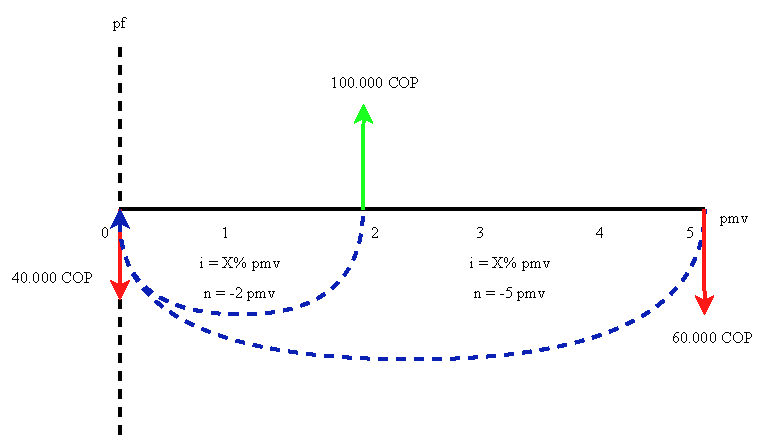
\includegraphics[scale=1]{ejemplos/4/Graf1Ej4Cap11.pdf} }
		\\\hline
		%%%%%%%%%%%%% FIN INSERCIÓN DE IMAGEN
		%%%%%FIN FLUJO DE CAJA



		%%%%% INICIO DECLARACIÓN FORMULAS
		%%%%%%%%%%% INICIO TITULO
		\rowcolor[HTML]{FFB183}
		\multicolumn{3}{|c|}{\cellcolor[HTML]{FFB183}\textbf{4. Declaración de fórmulas}}                                                                                                                                          \\ \hline
		%%%%%%%%%%% FIN TITULO
		%%%%%%%%%%% INICIO MATEMÁTICAS
		\multicolumn{3}{|c|} {VPN =	$\sum F_{n}(1+i)^{-n}$   Valor presente neto.}                                                                                                                                                 \\
		\multicolumn{3}{|c|} { $ i= j/m $ Tasa anualizada. }                                                                                                                                                                        \\

		\hline

		%%%%%%%%%% FIN MATEMÁTICAS
		%%%%%% INICIO DESARROLLO MATEMÁTICO
		\rowcolor[HTML]{FFB183}
		%%%%%%%%%%INICIO TITULO
		\multicolumn{3}{|c|}{\cellcolor[HTML]{FFB183}\textbf{5. Desarrollo matemático}}                                                                                                                                            \\ \hline
		%%%%%%%%%% FIN TITULO
		%%%%%%%%%% INICIO MATEMÁTICAS
		\multicolumn{3}{|c|}{-$40\text{.}000 COP   +  100\text{.}000 COP(1+i)^{-2}$ - $  60\text{.}000 COP(1+i)^{-5} = 0 COP$}
		\\

		\multicolumn{3}{|c|}{$ \text{Construimos una tabla de valores X,Y para ver el comportamiento de la gráfica y así determinar}$}
		\\
		\multicolumn{3}{|c|}{$ \text{las tasas:} $}
		\\

		\hline
		$ $                                                                       & \multicolumn{2}{c|}{ }                                                                                                                         \\

		{\fontsize{9}{10}\selectfont
		\setlength{\arrayrulewidth}{0.2mm} % Aumentar el grosor de las líneas
		\renewcommand{\arraystretch}{1.5} % Aumentar la altura de las filas
		\begin{tabular}{|>{\centering\arraybackslash}p{3cm}|>{\centering\arraybackslash}p{2cm}|}
			\hline
			\rowcolor{white!50}
			\textbf{X}     & \textbf{Y}  \\ \hline
			\text{0\%pmv}  & \text{0}    \\ \hline
			\text{10\%pmv} & \text{5,39} \\ \hline
			\text{20\%pmv} & \text{5,33} \\ \hline
			\text{30\%pmv} & \text{3,01} \\ \hline
			\text{40\%pmv} & \text{-135} \\ \hline
		\end{tabular}
		}
		                                                                          & \multicolumn{2}{c|}{{\fontsize{9}{10}\selectfont
					\setlength{\arrayrulewidth}{0.2mm} % Aumentar el grosor de las líneas
					\renewcommand{\arraystretch}{1.5} % Aumentar la altura de las filas
					\begin{tabular}{|>{\centering\arraybackslash}p{2cm}|>{\centering\arraybackslash}p{2cm}|}
						\hline
						\rowcolor{white!50}
						\textbf{X}     & \textbf{Y}      \\ \hline
						\text{39\%pmv} & \text{193,976}  \\ \hline
						\text{40\%pmv} & \text{-135,658} \\ \hline
					\end{tabular}
		}}                                                                                                                                                                                                                         \\
		$ $                                                                       & \multicolumn{2}{c|}{ }                                                                                                                         \\
		\hline
		\multicolumn{3}{|c|}{ }                                                                                                                                                                                                    \\

		\multicolumn{3}{|c|}{ \scalebox{1}{$\displaystyle\frac{39\%-40\%}{39\%-X} = \frac{193\text{,}976-(-135\text{,}658)}{193\text{,}975-0} $ }}
		\\
		\multicolumn{3}{|c|}{\text{Al despejar se obtiene el valor de X que es igual a 39,588 \% pmv}}                                                                                                                             \\
		\multicolumn{3}{|c|}{\text{Los resultados indican que existen dos tasas, pero no se sabe cuál escoger.}}
		\\
		\multicolumn{3}{|c|}{$ \text{Suponiendo una tasa del 30\% pmv para la reinversión, los ingresos serán:} $}
		\\
		\multicolumn{3}{|c|}{$ 100\text{.}000 COP(1 + 0.3)^{3} = $ $ 219\text{.}700 COP $}
		\\
		\multicolumn{3}{|c|}{$ 40\text{.}000 COP + 60\text{.}000 COP(1+0.25)^{-5} = $ $  59\text{.}660.80 COP $}                                                                                                                   \\ \hline
		\hline
		\multicolumn{3}{|c|}{$ \text{El nuevo diagrama de flujo de caja es:} $}
		\\
		\multicolumn{3}{|c|}{ 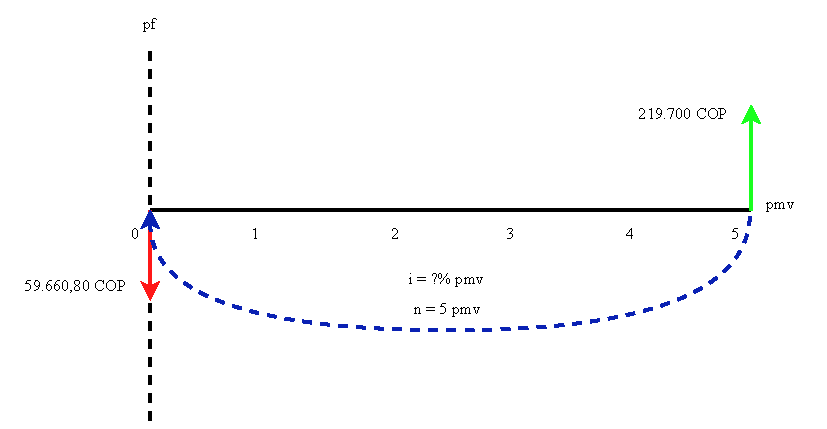
\includegraphics[scale=1]{ejemplos/4/Graf2Ej4Cap11.pdf} }
		\\
		\multicolumn{3}{|c|}{$ \text{Ahora se procede a calcular la TIRM:} $}
		\\
		\multicolumn{3}{|c|}{$219\text{.}700 COP = 59\text{.}660,80 COP(1+i)^{5} $}
		\\
		\multicolumn{3}{|c|}{$ TIRM = i = 29.786\% pmv $}
		\\
		\hline

		%%%%%%%%%% FIN MATEMÁTICAS
		%%%%%% FIN DESARROLLO MATEMÁTICO
		%%%%%% INICIO RESPUESTA
		\rowcolor[HTML]{FFB183}
		%%%%%%%%%%INICIO TITULO
		\multicolumn{3}{|c|}{\cellcolor[HTML]{FFB183}\textbf{6. Respuesta}}                                                                                                                                                        \\ \hline
		%%%%%%%%%% FIN TITULO
		%%%%%%%%%% INICIO RESPUESTA MATEMÁTICA

		\multicolumn{3}{|c|}{ \text{La TIRM del proyecto es igual a 29,786\% pmv}}
		\\

		\hline


		%%%%%%%%%% FIN MATEMÁTICAS
		%%%%%% FIN RESPUESTA
	\end{longtable}
	%Se crean dos lineas en blanco para que no quede el siguiente texto tan pegado
	%\newline \newline %USARLO SI CREES QUE ES NECESARIO
\end{center}
%%%%%%%%%%%%%%%%%%%%%%%%%%FIN EJERCICIO 1 %%%%%%%%%%%%%%%%%%%%%%%%%%%

